\documentclass[a4paper]{article}
\usepackage[german]{babel}
\usepackage[latin1]{inputenc}
\usepackage{color}
\usepackage{amsfonts}
%\usepackage{stmaryrd}
\usepackage{amsmath}
\usepackage{bm}
\usepackage{graphicx}
\usepackage{rotating}
\usepackage{pstricks}
\usepackage[top=1.75cm,bottom=1.75cm]{geometry}
%\setlength{\arraycolsep}{0mm}
\title{Graph Morphism Juggler}
\author{Martin Michels, Kornelius Walter}
\pagestyle{empty}
\newcommand{\Z}{\ensuremath{\mathbb{Z}}}
\newcommand{\N}{\ensuremath{\mathbb{N}}}
\newcommand{\mfA}{\ensuremath{{\mathfrak{A}}}}
\newcommand{\mfB}{\ensuremath{{\mathfrak{B}}}}
%\newcommand{\corona}{\lhd}
%\renewcommand{\diamond}{\diamondsuit}
%\newcommand{\boxcross}{\boxtimes}
%\newcommand{\complete}{\boxast}
\renewcommand{\phi}{\varphi}
\newcommand{\imp}{\ensuremath{\;\Rightarrow\;}}
\newcommand{\gdw}{\ensuremath{\;\Longleftrightarrow\;}}
\newenvironment{sm}{\left[\begin{smallmatrix}}{\end{smallmatrix}\right]}
\newcounter{cnt}
\begin{document}
\subsection*{Dokumentation}
\includegraphics[width=8cm]{main.ps}\\
The buttons in the upper bar from left to right are:
\begin{itemize}
\item New graph - this button opens a new window for a new graph
\item Add vertex - click on the button and then at the position where
  you want to add a vertex.
\item Add edge - click on the button and then on two vertices to add
  an edge between these two. (ToDo: Loops look stupid)
\item Fast save. If you don't want to overwrite the last ``fast
  saved'' graph, use ``Save graph'' from the menu and specify a
  filename. (The graph is saved in the file fastsavegraph.graph in the
  current working-directory.)
\item Fast load - loads the last ``fast saved'' graph.  Use ``Load
  graph'' from the menu for specifying a filename.
\item Zoom out.
\item Zoom in.
\item Print. Can print in a Postscript-File.
\item End - switches the cases, whether the program should examine
  endomorphisms or not.\\
  \includegraphics{end.ps} - Pressing the ``Card''-Button will analyse 
  the endomorphisms of the active graph.\\
  \includegraphics{noend.ps} -  Pressing the ``Card''-Button will ask 
  for two graphs, where the morphisms shall be analysed.
\item Info.
\item Quit.
\end{itemize}
The buttons in the left bar beginning with the top are:
\begin{itemize}
\item Card - Calculates cardinalities of isomorphisms, strong
  morphisms, quasi-strong morphisms, localy-strong morphisms,
  half-strong morphisms and homomorphisms (definitions are on the next
  page). If you examining endomorphisms, the program gives also the
  possibility to calculate some composition-tables and to test,
  whether HEnd, LEnd and QEnd are closed under composition.
\item Examine - Does nothing yet.
\item Combine - Computes the {\em Union}, {\em Join}, {\em Edge Join},
  {\em Cross Product} or {\em Box Product} of two graphs.
\item Factor graph - Computes the factor graph.
\end{itemize}
The buttons in the right bar beginning with the top are:
\begin{itemize}
\item More (up to now useless) information written in the vertices.
\item Directed / undirected graph.
\item Physics - A small force-based algorithm to arrange the vertices.
  At least good for looking, whether vertices are hidden under other vertices.
\end{itemize}

\end{document}
